%%%%%%%%%%%%%%%%%%%%%%%%%%%%%%%%%%%%%%%%%
% Beamer Presentation
% LaTeX Template
% Version 1.0 (10/11/12)
%
% This template has been downloaded from:
% http://www.LaTeXTemplates.com
%
% License:
% CC BY-NC-SA 3.0 (http://creativecommons.org/licenses/by-nc-sa/3.0/)
%
%%%%%%%%%%%%%%%%%%%%%%%%%%%%%%%%%%%%%%%%%

%----------------------------------------------------------------------------------------
%	PACKAGES AND THEMES
%----------------------------------------------------------------------------------------

\documentclass[UTF8,aspectratio=169,14pt]{ctexbeamer}

\usepackage{hyperref}
\hypersetup{
	colorlinks=true,
	linkcolor=red,
	anchorcolor=blue,
	citecolor=green
}

\mode<presentation> {
	
	% The Beamer class comes with a number of default slide themes
	% which change the colors and layouts of slides. Below this is a list
	% of all the themes, uncomment each in turn to see what they look like.
	
	%\usetheme{default}
	%\usetheme{AnnArbor}
	%\usetheme{Antibes}
	%\usetheme{Bergen}
	%\usetheme{Berkeley}
	%\usetheme{Berlin}
	%\usetheme{Boadilla}
	%\usetheme{CambridgeUS}
	%\usetheme{Copenhagen}
	%\usetheme{Darmstadt}
	%\usetheme{Dresden}
	%\usetheme{Frankfurt}
	%\usetheme{Goettingen}
	%\usetheme{Hannover}
	%\usetheme{Ilmenau}
	%\usetheme{JuanLesPins}
	%\usetheme{Luebeck}
	\usetheme{Madrid}
	%\usetheme{Malmoe}
	%\usetheme{Marburg}
	%\usetheme{Montpellier}
	%\usetheme{PaloAlto}
	%\usetheme{Pittsburgh}
	%\usetheme{Rochester}
	%\usetheme{Singapore}
	%\usetheme{Szeged}
	%\usetheme{Warsaw}
	
	% As well as themes, the Beamer class has a number of color themes
	% for any slide theme. Uncomment each of these in turn to see how it
	% changes the colors of your current slide theme.
	
	%\usecolortheme{albatross}
	%\usecolortheme{beaver}
	%\usecolortheme{beetle}
	%\usecolortheme{crane}
	%\usecolortheme{dolphin}
	%\usecolortheme{dove}
	%\usecolortheme{fly}
	%\usecolortheme{lily}
	%\usecolortheme{orchid}
	%\usecolortheme{rose}
	%\usecolortheme{seagull}
	%\usecolortheme{seahorse}
	%\usecolortheme{whale}
	%\usecolortheme{wolverine}
	
	%\setbeamertemplate{footline} % To remove the footer line in all slides uncomment this line
	%\setbeamertemplate{footline}[page number] % To replace the footer line in all slides with a simple slide count uncomment this line
	
	%\setbeamertemplate{navigation symbols}{} % To remove the navigation symbols from the bottom of all slides uncomment this line
}

\usepackage{graphicx} % Allows including images
\graphicspath{{./figs/}}
\usepackage{booktabs} % Allows the use of \toprule, \midrule and \bottomrule in tables
\usepackage{longtable}
\usepackage{listings}
\usepackage{xcolor}
\lstset{numbers=left, %设置行号位置
	numberstyle=\tiny, %设置行号大小
	keywordstyle=\color{blue}, %设置关键字颜色
	commentstyle=\color[cmyk]{1,0,1,0}, %设置注释颜色
	frame=single, %设置边框格式
	escapeinside=``, %逃逸字符(1左面的键),用于显示中文
	%breaklines, %自动折行
	extendedchars=false, %解决代码跨页时,章节标题,页眉等汉字不显示的问题
	xleftmargin=2em,xrightmargin=2em, aboveskip=1em, %设置边距
	tabsize=4, %设置tab空格数
	showspaces=false %不显示空格
}
% Fonts
% \usepackage{libertine}
% \setmonofont{Courier}
\setCJKsansfont[ItalicFont=Noto Serif CJK SC Black, BoldFont=Noto Sans CJK SC Black]{Noto Sans CJK SC}


%----------------------------------------------------------------------------------------
% TITLE PAGE
%----------------------------------------------------------------------------------------

\title[第21讲]{第二十一讲 :分布式系统} % The short title appears at the bottom of every slide, the full title is only on the title page
\subtitle{第2节:分布式文件系统}
\author{向勇、陈渝、李国良} % Your name
\institute[清华大学] % Your institution as it will appear on the bottom of every slide, may be shorthand to save space
{
    清华大学计算机系 \\ % Your institution for the title page
    \medskip
    \textit{xyong,yuchen,liguoliang@tsinghua.edu.cn} % Your email address
}
\date{\today} % Date, can be changed to a custom date

\begin{document}
    
    \begin{frame}
        \titlepage % Print the title page as the first slide
    \end{frame}
    
    %----------------------------------------------
    \begin{frame}
        \frametitle{提纲} % Table of contents slide, comment this block out to remove it
        \tableofcontents % Throughout your presentation, if you choose to use \section{} and \subsection{} commands, these will automatically be printed on this slide as an overview of your presentation
        
        %% itemize
        %Ref:
        %    \begin{itemize}
        %        \item \href{http://osq.cs.berkeley.edu/public/JFoster-Drivers.ppt}{Linux Device Drivers Overview}
        %        \item \href{http://ermak.cs.nstu.ru/understanding.linux.kernel.pdf}{Understanding the Linux Kernel}
        %    \end{itemize}
        
    \end{frame}
    %----------------------------------------------
    %%  PRESENTATION SLIDES
    %----------------------------------------------
    \section{第2节:分布式文件系统} % Sections can be created in order to organize your presentation into discrete blocks, all sections and subsections are automatically printed in the table of contents as an overview of the talk
    %----------------------------------------------
    \subsection{Sun的网络文件系统(NFS)} % A subsection can be created just before a set of slides with a common theme to further break down your presentation into chunks
    %----------------------------------------------
    \begin{frame}[fragile]
        \frametitle{分布式文件系统}
        分布式客户端/服务器计算的首次使用之一,是在分布式文件系统领域。
        
        关键问题:  如何构建分布式文件系统 
        
        对于客户端应用程序,分布式文件系统似乎与本地文件系统没有任何不同
        
        %    \framesubtitle{xxxx}
        %% figure
            \begin{figure}
            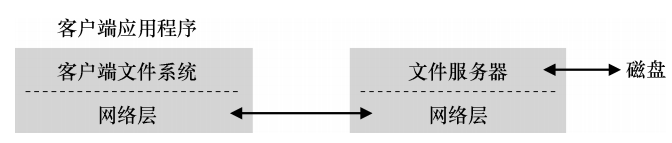
\includegraphics[width=0.8\linewidth]{figs/distributed-fs.png}
          %  \caption{xxxx}
            \end{figure}
    \end{frame}
%----------------------------------------------
\begin{frame}[fragile]
    \frametitle{Sun的NFS}
    %    \framesubtitle{xxxx}
    最早且相当成功的分布式系统之一是由Sun Microsystems开发的,被称为Sun网络文件系统(或NFS)
    \pause
    在定义NFS时,Sun开发了一种开放协议(open protocol),它只是指定了客户端和服务器用于通信的确切消息格式,而不是构建专有的封闭系统。
%    \begin{itemize}
%        \item 现代网络的核心原则是,通信基本是不可靠的。
%        \item 丢包是网络的基本现象
%        \item 应该如何处理丢包?
%    \end{itemize}
%http://bigdata-guide.blogspot.com/2014/02/network-file-system-nfs.html
        \begin{figure}
            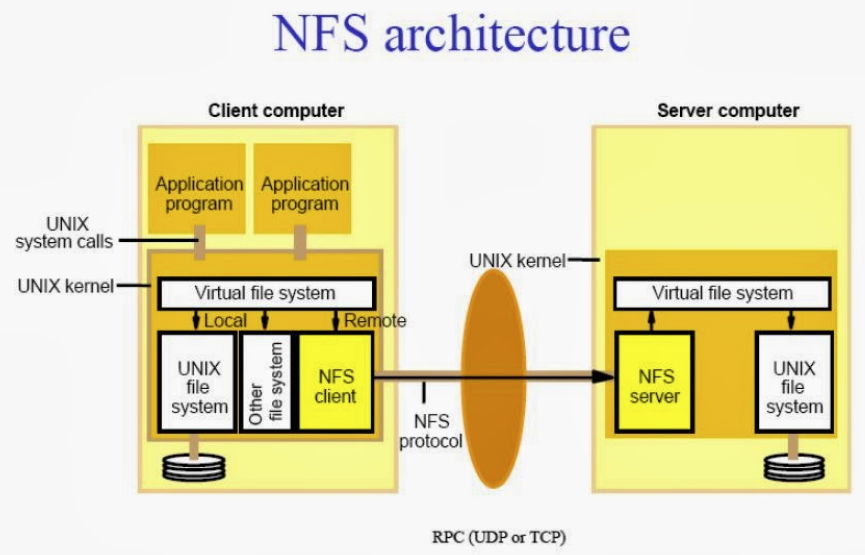
\includegraphics[width=0.5\linewidth]{figs/sun-nfs.png}
            %  \caption{xxxx}
        \end{figure}
\end{frame}
%----------------------------------------------
\begin{frame}[fragile]
    \frametitle{NFSv2协议}
%    \framesubtitle{xxxx}
关键技术
    \begin{itemize}
        \item 目标:简单快速的服务器崩溃恢复\pause
        \item 快速崩溃恢复的关键:无状态
        \item 简而言之,服务器不会追踪客户正在做什么
    \end{itemize}
    \begin{figure}
    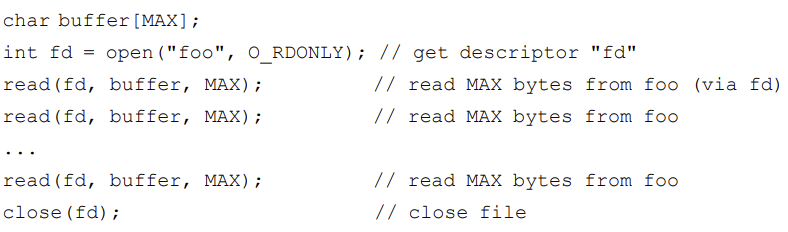
\includegraphics[width=0.8\linewidth]{figs/stateful-code.png}
    %  \caption{xxxx}
    \end{figure}
有状态(stateful)协议的示例。文件描述符是客户端和服务器之间的共享状态 
\end{frame}

%----------------------------------------------
\begin{frame}[fragile]
    \frametitle{NFSv2协议}
    %    \framesubtitle{xxxx}
    问题:共享状态使崩溃恢复变得复杂
    \begin{itemize}
        \item Srv:在第一次读取完成后,但在客户端发出第二次读取之前,服务器崩溃。
        \item Srv:服务器启动并再次运行后,客户端会发出第二次读取,但服务器不知道fd指的是哪个文件?
        \item Client:一个打开文件然后崩溃的客户端:open()在服务器上用掉了一个文件描述符,服务器如何关闭给定的文件呢?
    \end{itemize}
    \begin{figure}
        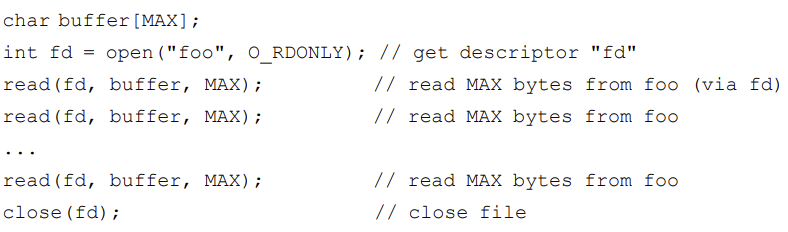
\includegraphics[width=0.8\linewidth]{figs/stateful-code.png}
        %  \caption{xxxx}
    \end{figure}

\end{frame}

%----------------------------------------------
\begin{frame}[fragile]
    \frametitle{NFSv2协议}
    %    \framesubtitle{xxxx}
    挑战:如何定义无状态文件协议,让它既无状态,又支持POSIX文件系统API?\pause
    \begin{itemize}
        \item 关键是文件句柄(file handle)。文件句柄用于唯一地描述文件或目录。因此,许多协议请求包括一个文件句柄。        
        \item 服务器启动并再次运行后,客户端会发出第二次读取,但服务器不知道fd指的是哪个文件?
        \item 一个打开文件然后崩溃的客户端:open()在服务器上用掉了一个文件描述符,服务器如何关闭给定的文件呢?
    \end{itemize}
    \begin{figure}
        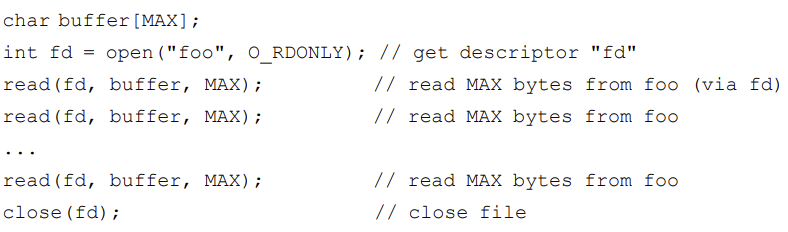
\includegraphics[width=0.8\linewidth]{figs/stateful-code.png}
        %  \caption{xxxx}
    \end{figure}
    
\end{frame}


%----------------------------------------------
\begin{frame}[fragile]
    \frametitle{NFSv2协议}
    %    \framesubtitle{xxxx}
%    挑战:如何定义无状态文件协议,让它既无状态,又支持POSIX文件系统API?
%    \begin{itemize}
%        \item 关键是文件句柄(file handle)。文件句柄用于唯一地描述文件或目录。因此,许多协议请求包括一个文件句柄。        
%        \item 2. 服务器启动并再次运行后,客户端会发出第二次读取,但服务器不知道fd指的是哪个文件?
%        \item 1. 一个打开文件然后崩溃的客户端:open()在服务器上用掉了一个文件描述符,服务器如何关闭给定的文件呢?
%    \end{itemize}
NFSv2协议 part1
    \begin{figure}
        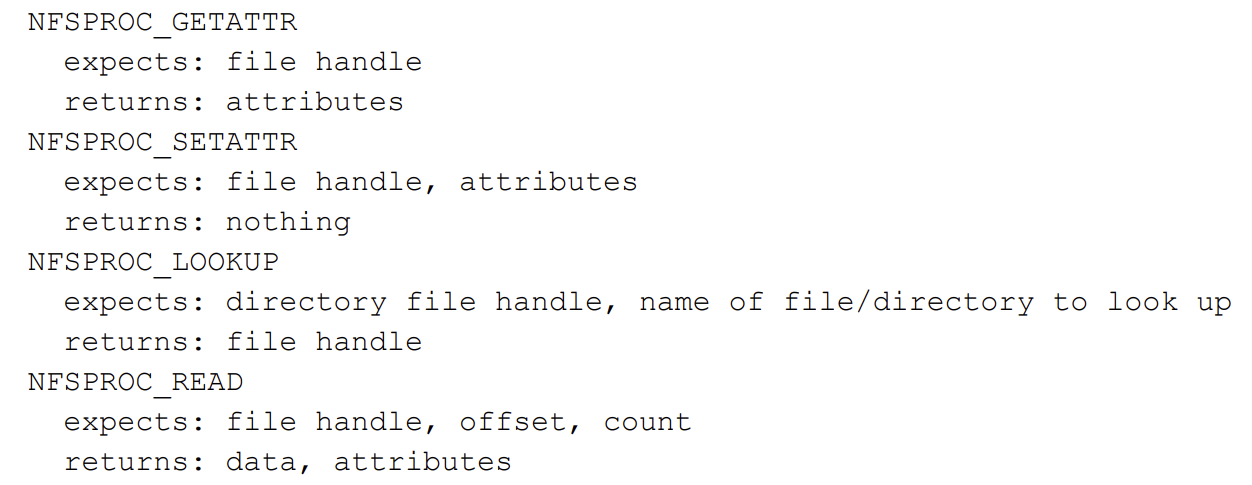
\includegraphics[width=0.9\linewidth]{figs/nfsv2-1.png}
        %  \caption{xxxx}
    \end{figure}
    
\end{frame}
%----------------------------------------------
\begin{frame}[fragile]
    \frametitle{NFSv2协议}
    %    \framesubtitle{xxxx}
    %    挑战:如何定义无状态文件协议,让它既无状态,又支持POSIX文件系统API?
    %    \begin{itemize}
    %        \item 关键是文件句柄(file handle)。文件句柄用于唯一地描述文件或目录。因此,许多协议请求包括一个文件句柄。        
    %        \item 2. 服务器启动并再次运行后,客户端会发出第二次读取,但服务器不知道fd指的是哪个文件?
    %        \item 1. 一个打开文件然后崩溃的客户端:open()在服务器上用掉了一个文件描述符,服务器如何关闭给定的文件呢?
    %    \end{itemize}
    NFSv2协议 part2
    \begin{figure}
        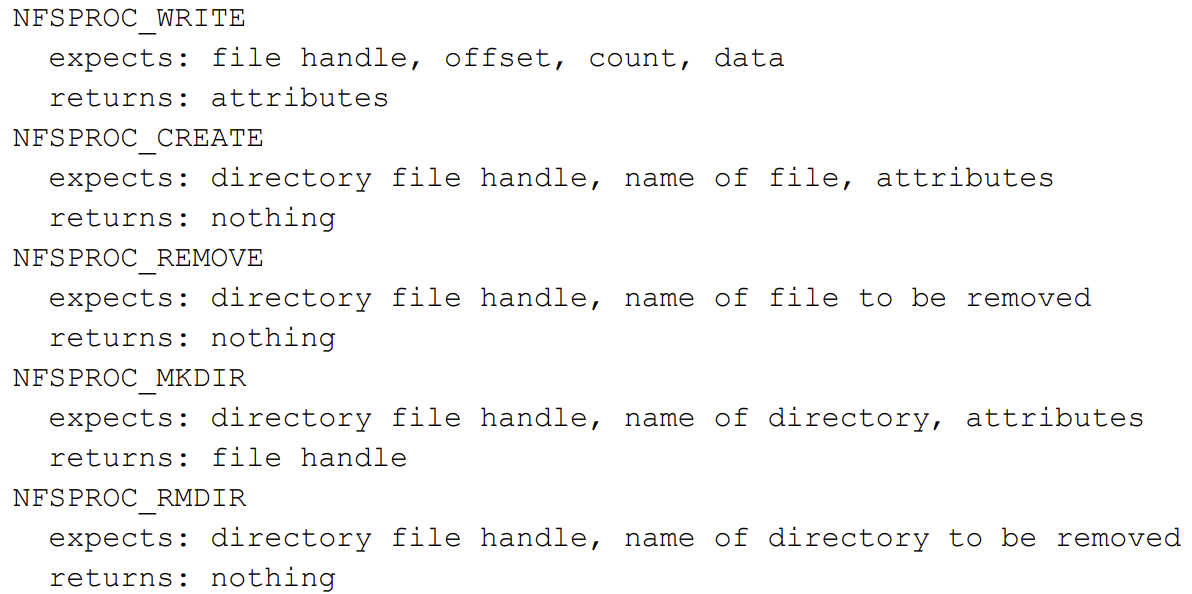
\includegraphics[width=0.8\linewidth]{figs/nfsv2-2.png}
        %  \caption{xxxx}
    \end{figure}
    
\end{frame}


%----------------------------------------------
\begin{frame}[fragile]
    \frametitle{NFSv2协议}
    %    \framesubtitle{xxxx}
    %    挑战:如何定义无状态文件协议,让它既无状态,又支持POSIX文件系统API?
    %    \begin{itemize}
    %        \item 关键是文件句柄(file handle)。文件句柄用于唯一地描述文件或目录。因此,许多协议请求包括一个文件句柄。        
    %        \item 2. 服务器启动并再次运行后,客户端会发出第二次读取,但服务器不知道fd指的是哪个文件?
    %        \item 1. 一个打开文件然后崩溃的客户端:open()在服务器上用掉了一个文件描述符,服务器如何关闭给定的文件呢?
    %    \end{itemize}
    读取文件:客户端和文件服务器的操作 part1
    \begin{figure}
        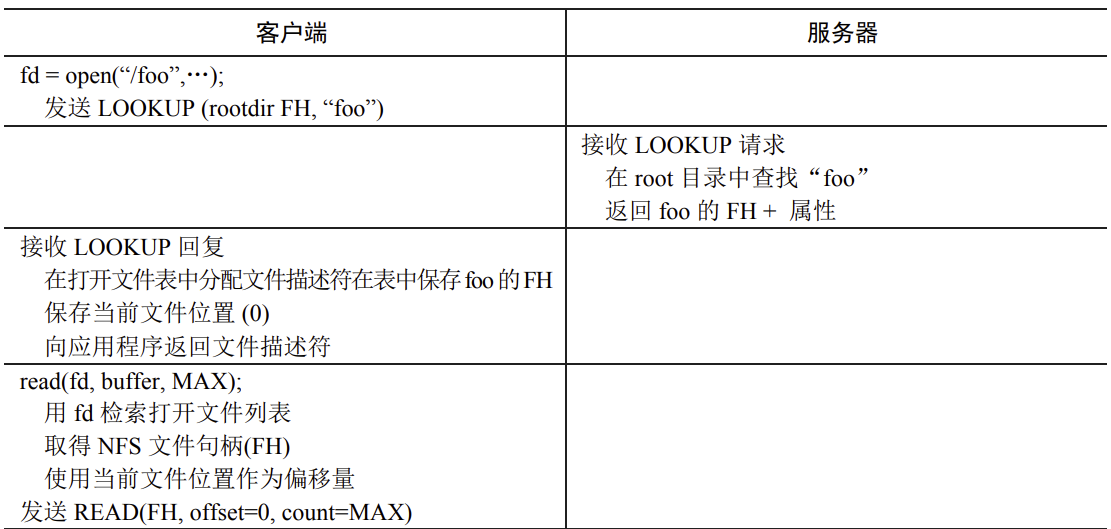
\includegraphics[width=0.8\linewidth]{figs/nfsv2-read-1.png}
        %  \caption{xxxx}
    \end{figure}
    
\end{frame}

%----------------------------------------------
\begin{frame}[fragile]
    \frametitle{NFSv2协议}
    %    \framesubtitle{xxxx}
    %    挑战:如何定义无状态文件协议,让它既无状态,又支持POSIX文件系统API?
    %    \begin{itemize}
    %        \item 关键是文件句柄(file handle)。文件句柄用于唯一地描述文件或目录。因此,许多协议请求包括一个文件句柄。        
    %        \item 2. 服务器启动并再次运行后,客户端会发出第二次读取,但服务器不知道fd指的是哪个文件?
    %        \item 1. 一个打开文件然后崩溃的客户端:open()在服务器上用掉了一个文件描述符,服务器如何关闭给定的文件呢?
    %    \end{itemize}
    读取文件:客户端和文件服务器的操作 part2
    \begin{figure}
        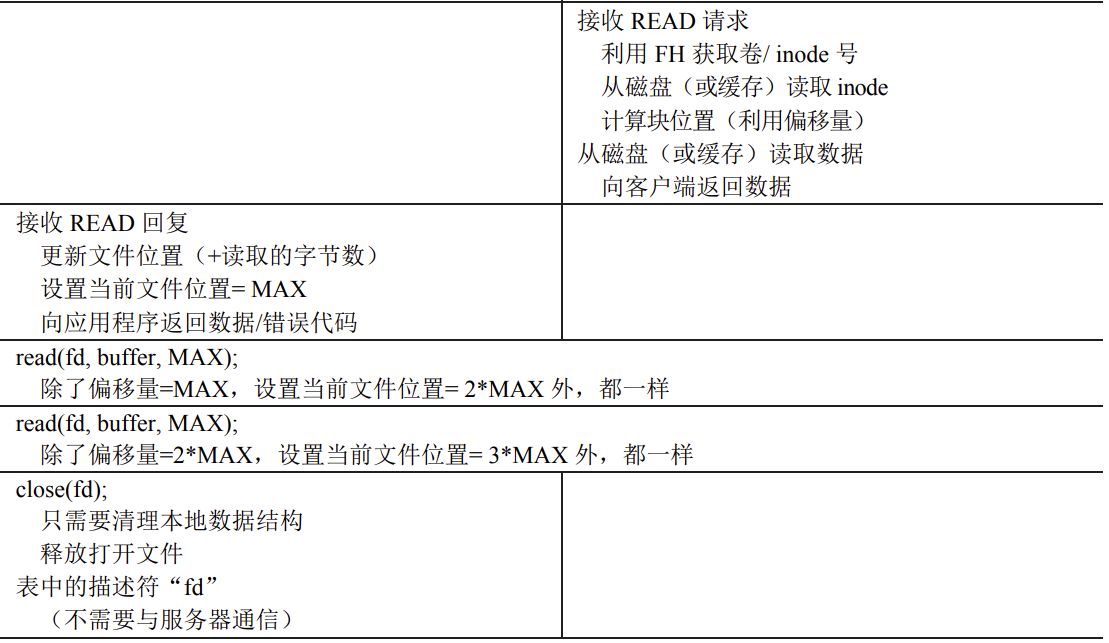
\includegraphics[width=0.7\linewidth]{figs/nfsv2-read-2.png}
        %  \caption{xxxx}
    \end{figure}
    
\end{frame}

%----------------------------------------------
\begin{frame}[fragile]
    \frametitle{NFSv2协议}
    %    \framesubtitle{xxxx}
    幂等性

        \begin{itemize}
            \item 如果操作执行多次的效果与执行一次的效果相同,该操作就是幂等的(idempotent)  \pause
            \item 如果将值在内存位置存储 3 次,与存储一次一样。因此“将值存储到内存中”是一种幂等操作。
            \item 如果将计数器递增 3 次,它的数量就会与递增一次不同。
            \item LOOKUP和READ请求是简单幂等的,因为它们只从文件服务器读取信息而不更新它。
            \item WRITE请求也是幂等的。WRITE消息包含数据、计数和(重要的)写入数据的确切偏移量。因此,可以重复多次写入,因为多次写入的结果与单次的结果相同。
        \end{itemize}
    
%    \begin{figure}
%        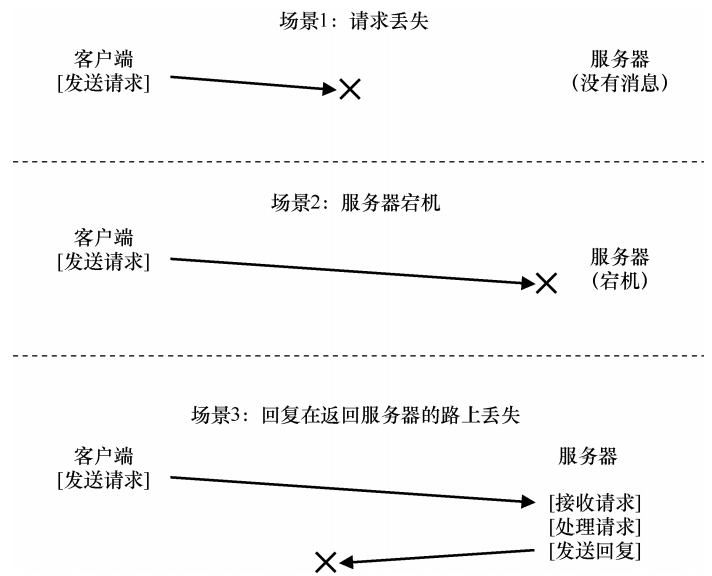
\includegraphics[width=0.5\linewidth]{figs/nfsv2-lose.png}
%        %  \caption{xxxx}
%    \end{figure}
    
\end{frame}

%----------------------------------------------
\begin{frame}[fragile]
    \frametitle{NFSv2协议}
    %    \framesubtitle{xxxx}
    %    挑战:如何定义无状态文件协议,让它既无状态,又支持POSIX文件系统API?
    %    \begin{itemize}
    %        \item 关键是文件句柄(file handle)。文件句柄用于唯一地描述文件或目录。因此,许多协议请求包括一个文件句柄。        
    %        \item 2. 服务器启动并再次运行后,客户端会发出第二次读取,但服务器不知道fd指的是哪个文件?
    %        \item 1. 一个打开文件然后崩溃的客户端:open()在服务器上用掉了一个文件描述符,服务器如何关闭给定的文件呢?
    %    \end{itemize}
    利用幂等操作处理服务器故障 (3种类型的丢失)
    \begin{figure}
        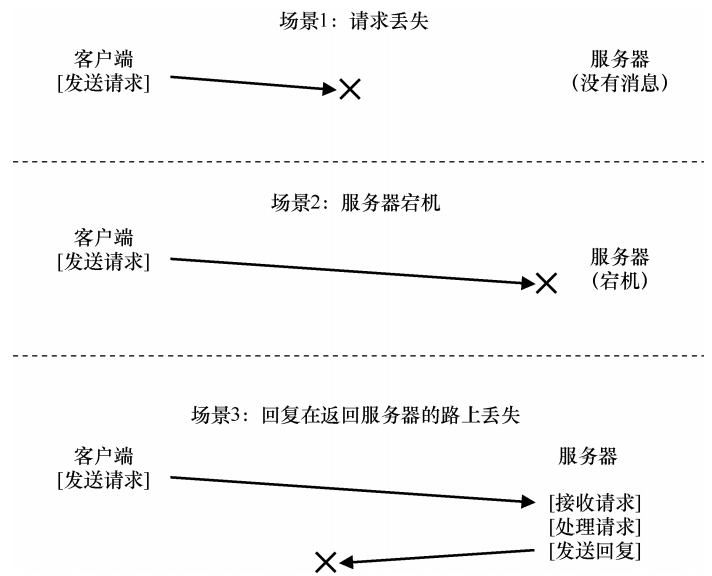
\includegraphics[width=0.5\linewidth]{figs/nfsv2-lose.png}
        %  \caption{xxxx}
    \end{figure}
    
\end{frame}

%----------------------------------------------
\begin{frame}[fragile]
    \frametitle{NFSv2协议}
    %    \framesubtitle{xxxx}
    客户端以统一的幂等操作方式处理了消息丢失和服务器故障
    
    \begin{itemize}
        \item 如果WRITE请求丢失(上面的第一种情况),客户端将重试它,服务器将执行写入,一切都会好。 
        \item 如果在请求发送时,服务器恰好关闭,但在第二个请求发送时,服务器已重启并继续运行,则又会如愿执行(第二种情况)。
        \item 服务器可能实际上收到了WRITE请求,发出写入磁盘并发送回复。此回复可能会丢失(第三种情况),导致客户端重新发送请求。当服务器再次收到请求时,它就会执行相同的操作:将数据写入磁盘,并回复它已完成该操作。如果客户端这次收到了回复,则一切正常
    \end{itemize}
    一些操作(mkdir)很难成为幂等的
    %    \begin{figure}
    %        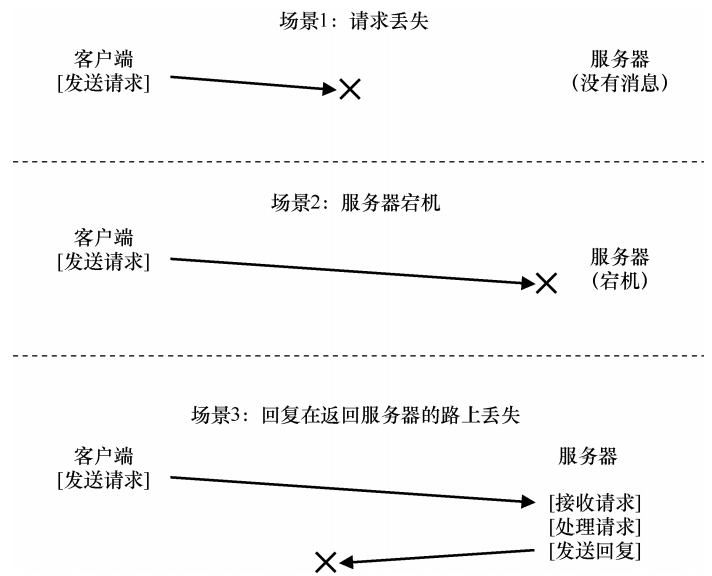
\includegraphics[width=0.5\linewidth]{figs/nfsv2-lose.png}
    %        %  \caption{xxxx}
    %    \end{figure}
    
\end{frame}


%----------------------------------------------
\begin{frame}[fragile]
    \frametitle{NFSv2协议}
    %    \framesubtitle{xxxx}
    提高性能:客户端缓存
    
    \begin{itemize}
        \item NFS客户端文件系统缓存文件数据(和元数据)
        \item 缓存还可用作写入的临时缓冲区
    \end{itemize}

        \begin{figure}
            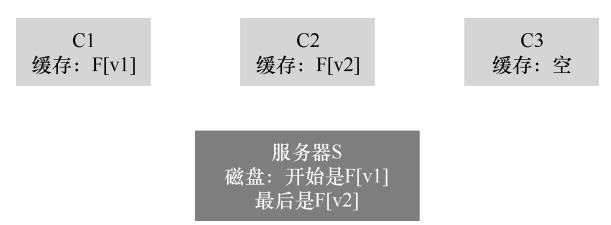
\includegraphics[width=0.7\linewidth]{figs/nfsv2-cache.png}
            %  \caption{xxxx}
        \end{figure}
    
\end{frame}

%----------------------------------------------
\begin{frame}[fragile]
    \frametitle{NFSv2协议}
    %    \framesubtitle{xxxx}
    潜在问题:缓存一致性问题
    
    \begin{itemize}
        \item “更新可见性(update visibility)”问题:来自一个客户端的更新,什么时候被其他客户端看见?\pause
        \item “陈旧的缓存(stale cache)“问题:C2最终将它的写入发送给文件服务器,因此服务器具有最新版本(F[v2])。但是,C1的缓存中仍然是F[v1]。如果运行在C1上的程序读了文件F,它将获得过时的版本(F [v1]),而不是最新的版本(F [v2])
    \end{itemize}
    
    \begin{figure}
        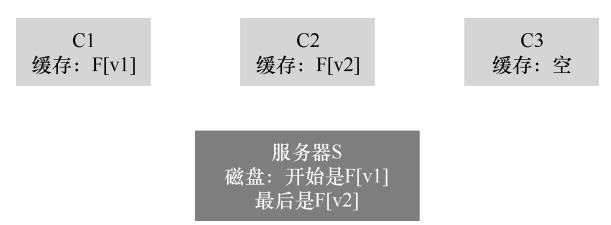
\includegraphics[width=0.5\linewidth]{figs/nfsv2-cache.png}
        %  \caption{xxxx}
    \end{figure}
    
\end{frame}


%----------------------------------------------
\begin{frame}[fragile]
    \frametitle{NFSv2协议}
    %    \framesubtitle{xxxx}
    解决方法:缓存一致性问题
    
    “更新可见性(update visibility)”问题:一个客户端的更新何时被其他客户端看见?
    \begin{itemize}
        \item 客户端实现称为“关闭时刷新”(flush-on-close,即close-to-open)的一致性语义。具体来说,当应用程序写入文件并随后关闭文件时,客户端将所有更新(即缓存中的脏页面)刷新到服务器。通过关闭时刷新的一致性,NFS可确保后续从另一个节点打开文件,会看到最新的文件版本。
    \end{itemize}
    
    \begin{figure}
        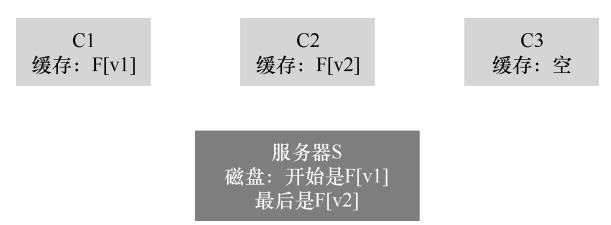
\includegraphics[width=0.5\linewidth]{figs/nfsv2-cache.png}
        %  \caption{xxxx}
    \end{figure}
    
\end{frame}

%----------------------------------------------
\begin{frame}[fragile]
    \frametitle{NFSv2协议}
    %    \framesubtitle{xxxx}
    潜在问题:缓存一致性问题
    
    “陈旧的缓存(stale cache)“问题:C2最终将它的写入发送给文件服务器,因此服务器具有最新版本(F[v2])。但是,C1的缓存中仍然是F[v1]。如果运行在C1上的程序读了文件F,它将获得过时的版本(F [v1]),而不是最新的版本(F [v2])\pause
    \begin{itemize}
        \item NFSv2客户端会先检查文件是否已更改,然后再使用其缓存内容。具体来说,在打开文件时,客户端文件系统会发出GETATTR请求,以获取文件的属性。
        \item 属性包含有关服务器上次修改文件的信息。如果文件修改的时间晚于文件提取到客户端缓存的时间,则客户端会让文件无效(invalidate),因此将它从客户端缓存中删除,并确保后续的读取将转向服务器,取得该文件的最新版本。
    \end{itemize}
    
%    \begin{figure}
%        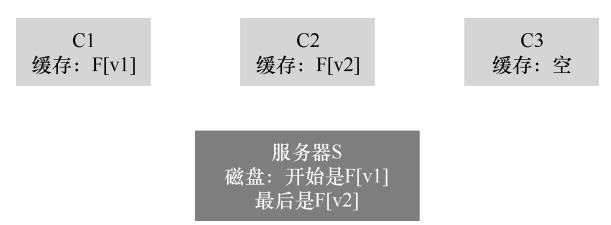
\includegraphics[width=0.5\linewidth]{figs/nfsv2-cache.png}
%        %  \caption{xxxx}
%    \end{figure}
    
\end{frame}


%----------------------------------------------
\begin{frame}[fragile]
    \frametitle{NFSv2协议}
    %    \framesubtitle{xxxx}
    潜在问题:服务器端写缓冲问题\pause
    
    客户端发出以下写入序列
%    \begin{itemize}
%        \item NFSv2客户端会先检查文件是否已更改,然后再使用其缓存内容。具体来说,在打开文件时,客户端文件系统会发出GETATTR请求,以获取文件的属性。
%        \item 属性包含有关服务器上次修改文件的信息。如果文件修改的时间晚于文件提取到客户端缓存的时间,则客户端会让文件无效(invalidate),因此将它从客户端缓存中删除,并确保后续的读取将转向服务器,取得该文件的最新版本。
%    \end{itemize}
    
        \begin{figure}
            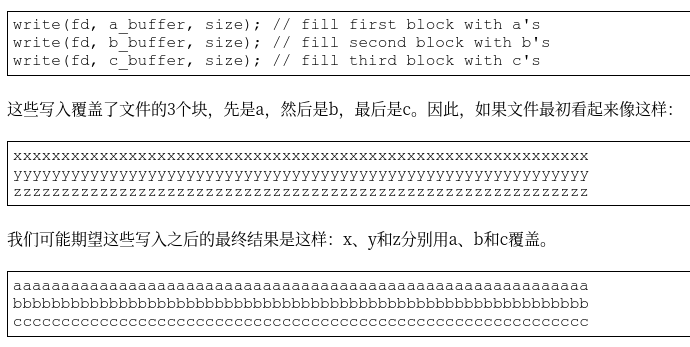
\includegraphics[width=.8\linewidth]{figs/nfsv2-srv1.png}
            %  \caption{xxxx}
        \end{figure}
    
\end{frame}

%----------------------------------------------
\begin{frame}[fragile]
    \frametitle{NFSv2协议}
    %    \framesubtitle{xxxx}
    潜在问题:服务器端写缓冲问题
    
    假设服务器接收到第一个WRITE消息,将它发送到磁盘,并向客户端通知成功。现在假设第二次写入只是缓冲在内存中,服务器在强制写入磁盘之前,也向客户端报告成功。但服务器在写入磁盘之前崩溃了。服务器快速重启,并接收第三个写请求,该请求也成功了。
    
    因此,对于客户端,所有请求都成功了,但文件的内容如下:
    %    \begin{itemize}
    %        \item NFSv2客户端会先检查文件是否已更改,然后再使用其缓存内容。具体来说,在打开文件时,客户端文件系统会发出GETATTR请求,以获取文件的属性。
    %        \item 属性包含有关服务器上次修改文件的信息。如果文件修改的时间晚于文件提取到客户端缓存的时间,则客户端会让文件无效(invalidate),因此将它从客户端缓存中删除,并确保后续的读取将转向服务器,取得该文件的最新版本。
    %    \end{itemize}
    
    \begin{figure}
        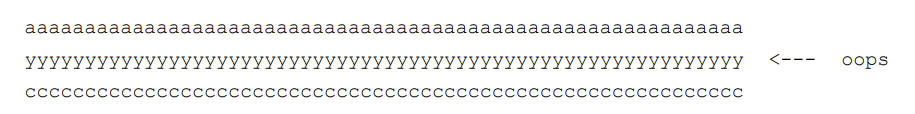
\includegraphics[width=0.9\linewidth]{figs/nfsv2-srv2.png}
        %  \caption{xxxx}
    \end{figure} \pause
    
    解决方法:NFS服务器在通知客户端成功之前,将每次写入提交到持久存储。这样做可让客户端在写入期间检测到服务器故障,从而重试,直到它最终成功。
\end{frame}

%----------------------------------------------
\begin{frame}[fragile]
    \frametitle{NFSv2协议 -- 小结}
    %    \framesubtitle{xxxx}
    
        \begin{itemize}
            \item NFS的核心:服务器的故障要能简单快速地恢复。
            \item 文件操作的幂等性至关重要,因为客户端可以安全地重试失败的操作,不论服务器是否已执行该请求,都可以这样做。
            \item 将缓存引入多客户端、单服务器的系统,如何会让事情变得复杂。系统必须解决缓存一致性问题,才能合理地运行。
            
            
        \end{itemize}
    
%    \begin{figure}
%        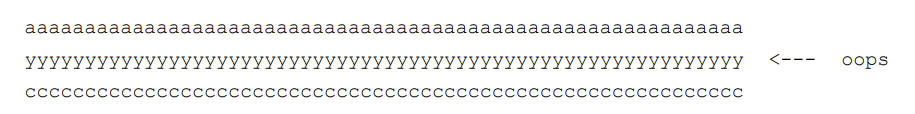
\includegraphics[width=0.9\linewidth]{figs/nfsv2-srv2.png}
%        %  \caption{xxxx}
%    \end{figure}
%    
%    解决方法:NFS服务器在通知客户端成功之前,将每次写入提交到持久存储。这样做可让客户端在写入期间检测到服务器故障,从而重试,直到它最终成功。
\end{frame}
%----------------------------------------------
\end{document}
